\section{简单的磁现象}\label{sec:10-1}

春秋战国时期,我们的祖先就发现有的铁矿石能够吸引铁质物体。这种矿石叫做天然磁铁。

把磁铁靠近用不同材料制成的物体,发现磁铁只能吸引铁、钴、镍等物质。
我们把物体能够吸引铁、钴、镍等物质的性质叫做\textbf{磁性}。具有磁性的物体叫做\textbf{磁体}。

能够长期保持磁性的磁体叫做永磁体。永磁体有天然磁体和人造磁体两种。
人造磁体通常是用钢或某些合金制成的,根据需要可以加工成条形、针形、蹄形等各种形状(图 \ref{fig:10-1})。

\begin{figure}[htbp]
    \centering
    \begin{minipage}{7cm}
    \centering
    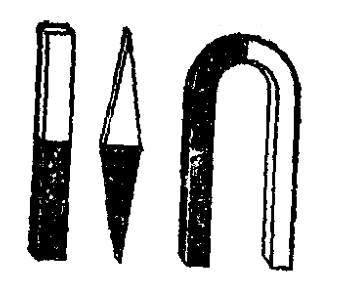
\includegraphics[width=5cm]{../pic/czwl2-ch10-1}
    \caption{常用的几种形状的永磁体}\label{fig:10-1}
    \end{minipage}
    \qquad
    \begin{minipage}{7cm}
    \centering
    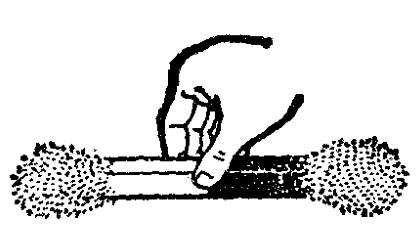
\includegraphics[width=6cm]{../pic/czwl2-ch10-2}
    \caption{显示条形磁铁的磁极}\label{fig:10-2}
    \end{minipage}
\end{figure}

把一根条形磁铁放在铁屑里再拿出来,可以看到条形磁铁两端吸的铁屑最多,中间最少(图 \ref{fig:10-2})。
这表明条形磁铁两端的磁性最强,中间最弱。磁体上磁性最强的部分叫做\textbf{磁极}。


\begin{figure}[htbp]
    \centering
    \begin{minipage}{7cm}
    \centering
    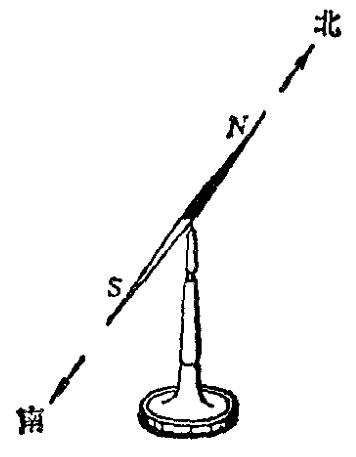
\includegraphics[width=4cm]{../pic/czwl2-ch10-3}
    \caption{}\label{fig:10-3}
    \end{minipage}
    \qquad
    \begin{minipage}{7cm}
    \centering
    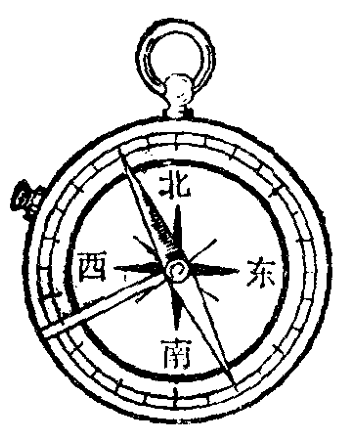
\includegraphics[width=4cm]{../pic/czwl2-ch10-4}
    \caption{}\label{fig:10-4}
    \end{minipage}
\end{figure}

把磁针支在针尖上面,使它能在水平面内自由转动,当它停下来的时候,总是一个磁极指南,另一个磁极指北(图 \ref{fig:10-3})。
如果把条形磁铁吊起来,使它能在水平面内自由转动,也会看到同样的现象。磁铁
指南的那个磁极叫\textbf{南极},用 $S$ 表示;
指北的那个磁极叫\textbf{北极},用 $N$ 表示。


磁铁指南北的性质可以用来制成指南针。现代的指南针(罗盘)是用人造磁铁制成的,形状如图 \ref{fig:10-4} 所示。

把条形磁铁的北极靠近磁针的北极,可以看到它们互相推斥;
把条形磁铁的南极靠近磁针的北极,可以看到它们互相吸引(图 \ref{fig:10-5})。
这表明\textbf{同名磁极互相推斥,异名磁极互相吸引}。

\begin{figure}[htbp]
    \centering
    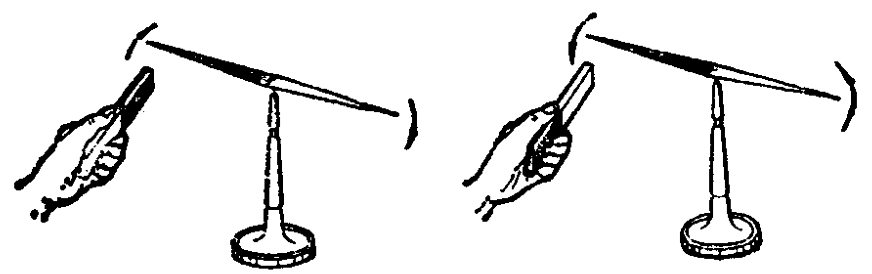
\includegraphics[width=0.8\textwidth]{../pic/czwl2-ch10-5}
    \caption{磁极间的相互作用}\label{fig:10-5}
\end{figure}


图 \ref{fig:10-6} 甲中的铁棒原来没有磁性,不吸引铁屑,但是当一根磁铁靠近它时,
它在磁铁的作用下获得了磁性(图 \ref{fig:10-6} 乙)。
这种使原来没有磁性的物体得到磁性的过程叫做\textbf{磁化}。
在图 \ref{fig:10-6} 乙的实验中,如果把磁铁拿开,被磁化的铁棒的磁性差不多完全消失。
如果被磁化的不是铁棒而是钢棒,那么磁铁拿开后钢棒仍有磁性。
钢有保持磁性的性质,因此常用钢来制造永磁体。

\begin{figure}[htbp]
    \centering
    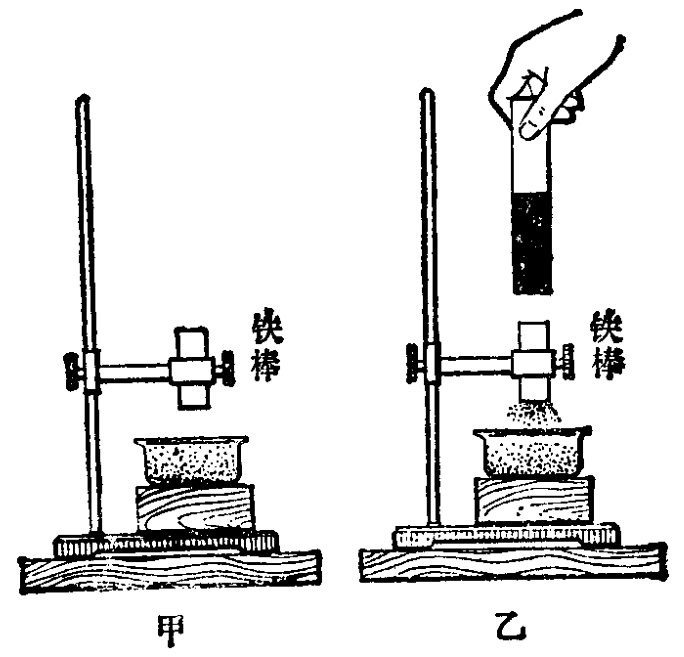
\includegraphics[width=0.6\textwidth]{../pic/czwl2-ch10-6}
    \caption{}\label{fig:10-6}
\end{figure}


\section*{阅读材料}

我国最早有关磁石的记载,见于春秋战国时期的《管子·地数》篇,里面有
“上有慈石\footnote{古书里的 “慈石”,就是现在的 “磁石”。} 者,其下有铜金” 的说法。
其后在不少古书中,还有许多关于磁石的记载。
例如,在公元前三世纪的战国时代,有一部《吕氏春秋》,有 “慈石召铁” 的记载。
在一些古书里,还记了关于磁石的有趣的传说。
例如,秦始皇为了防刺客而用磁石来修建阿房宫的大门,据说这样身披铁甲暗藏利刃的刺客,到了门前就会被吸住。

\begin{figure}[htbp]
    \centering
    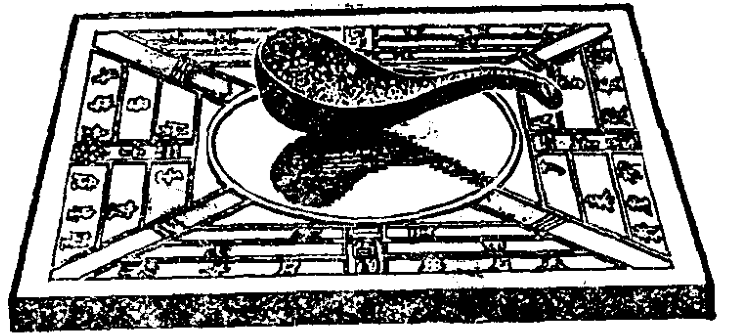
\includegraphics[width=0.4\textwidth]{../pic/czwl2-ch10-7}
    \caption{司南模型}\label{fig:10-7}
\end{figure}

大约在公元前三世纪,我国人民就发现了磁铁指南北的性质,并制成了世界上最早的指南工具“司南”。
它是用天然磁石琢磨而成的勺子,放在刻有方位的铜盘上(图 \ref{fig:10-7})。
用手拨动一下勺子,当勺子静止下来的时候,勺柄指南,勺头指北。

“司南” 制造起来相当麻烦,由于勺跟盘之间的摩擦,准确度也较差。
我国人民经过长时期的探索,发现钢与天然磁石接触后,也有了磁性,并且磁能够长期保持,
于公元十一世纪把钢做成针状,用天然磁石使它磁化,制成了人造的指南针。
指南针制作简便,又相当灵敏,这比起司南是个进步。

指南针是中国古代的四大发明之一。
宋朝时候,我国做买卖的大海船利用指南针导航,往来于我国和南洋群岛、印度之间。
阿拉伯商人和波斯商人,经常搭乘我国的海船,也学会了使用指南针。
过了若干年,他们又把指南针传入欧洲。指南针的发明,推动了航海事业的发展,
促进了世界经济和文化的交流,对人类的进步作出了贡献。

